% !TEX TS-program = pdflatex
% !TEX encoding = UTF-8 Unicode

% This is a simple template for a LaTeX document using the "article" class.
% See "book", "report", "letter" for other types of document.

\documentclass[11pt]{article} % use larger type; default would be 10pt
\usepackage[spanish]{babel}
\usepackage[utf8]{inputenc} % set input encoding (not needed with XeLaTeX)
\usepackage{ctable}
\usepackage{sectsty}
\usepackage[all]{xy}
%%% Examples of Article customizations
% These packages are optional, depending whether you want the features they provide.
% See the LaTeX Companion or other references for full information.
%%% PAGE DIMENSIONS
\usepackage{geometry} % to change the page dimensions
\geometry{a4paper} % or letterpaper (US) or a5paper or....
% \geometry{margin=2in} % for example, change the margins to 2 inches all round
% \geometry{landscape} % set up the page for landscape
%   read geometry.pdf for detailed page layout information
\usepackage[rightcaption]{sidecap}
\usepackage{graphicx} % support the \includegraphics command and options
\usepackage{amsmath}
\usepackage{amsfonts}
% \usepackage[parfill]{parskip} % Activate to begin paragraphs with an empty line rather than an indent

%%% PACKAGES
\usepackage{booktabs} % for much better looking tables
\usepackage{listings}
\usepackage{array} % for better arrays (eg matrices) in maths
\usepackage{paralist} % very flexible & customisable lists (eg. enumerate/itemize, etc.)
\usepackage{verbatim} % adds environment for commenting out blocks of text & for better verbatim
\usepackage{subfig} % make it possible to include more than one captioned figure/table in a single float
% These packages are all incorporated in the memoir class to one degree or another...
\usepackage{amsfonts}
\usepackage{amsmath,amssymb}
\usepackage{graphicx}
\usepackage{listings}
%%% HEADERS & FOOTERS
\usepackage{fancyhdr} % This should be set AFTER setting up the page geometry
\pagestyle{fancy} % options: empty , plain , fancy
\renewcommand{\headrulewidth}{0pt} % customise the layout...
\lhead{}\chead{}\rhead{}
\lfoot{}\cfoot{\thepage}\rfoot{}
\usepackage[T1]{fontenc}
%%% SECTION TITLE APPEARANCE
\usepackage{sectsty}
\allsectionsfont{\sffamily\mdseries\upshape} % (See the fntguide.pdf for font help)
% (This matches ConTeXt defaults)
\usepackage[ruled,vlined]{algorithm2e}
%%% ToC (table of contents) APPEARANCE
\usepackage[nottoc,notlof,notlot]{tocbibind} % Put the bibliography in the ToC
\usepackage[titles,subfigure]{tocloft} % Alter the style of the Table of Contents
\renewcommand{\cftsecfont}{\rmfamily\mdseries\upshape}
\renewcommand{\cftsecpagefont}{\rmfamily\mdseries\upshape} % No bold!

%%% END Article customizations
% ==========================
% = Matemáticas y teoremas =
% ==========================
\usepackage[]{amsmath}
\usepackage[]{amsthm}
\usepackage[]{mathtools}
\usepackage[]{bm}
\usepackage[]{thmtools}
\newcommand{\marcador}{\vrule height 10pt depth 2pt width 2pt \hskip .5em\relax}
\newcommand{\cabeceraespecial}{%
	
	\normalfont\bfseries}
\declaretheoremstyle[
spaceabove=\medskipamount,
spacebelow=\medskipamount,
headfont=\cabeceraespecial\marcador,
notefont=\cabeceraespecial,
notebraces={(}{)},
bodyfont=\normalfont\itshape,
postheadspace=1em,
numberwithin=section,
headindent=0pt,
headpunct={.}
]{importante}
\declaretheoremstyle[
spaceabove=\medskipamount,
spacebelow=\medskipamount,
headfont=\normalfont\itshape,
notefont=\normalfont,
notebraces={(}{)},
bodyfont=\normalfont,
postheadspace=1em,
numberwithin=section,
headindent=0pt,
headpunct={.}
]{normal}
% Los nombres de los enunciados. Añade los que necesites.
\declaretheorem[name=Observaci\'on, style=normal]{remark}

\declaretheorem[name=Corolario, style=normal]{corollary}

\declaretheorem[name=Proposici\'on, style=normal]{proposition}

\declaretheorem[name=Lema, style=normal]{lemma}

\declaretheorem[name=Ejemplo , style=definition, numberwithin=section]{ejemplo}


\declaretheorem[name=Teorema, style=importante]{theorem}

\declaretheorem[name=Definici\'on, style=importante]{definition}



%%% The "real" document content comes below...
\title{Análisis de sentimientos multimodal}
\author{Sara Olías Zapico}

\begin{document}
	\maketitle
\renewcommand{\refname}{Bibliografía}

\tableofcontents

\newpage

\section{Fundamentos teóricos}

\subsection{Redes neuronales}

Las redes neuronales, surgen de la idea de imitar las redes biológicas para solucionar problemas de inteligencia artificial. Estas redes artificiales han ido evolucionando y se han diseñado variaciones para cada tipo de problema

A nivel esquemático, una neurona artificial se representa del siguiente modo:


\begin{figure}[h!]
	\centering
	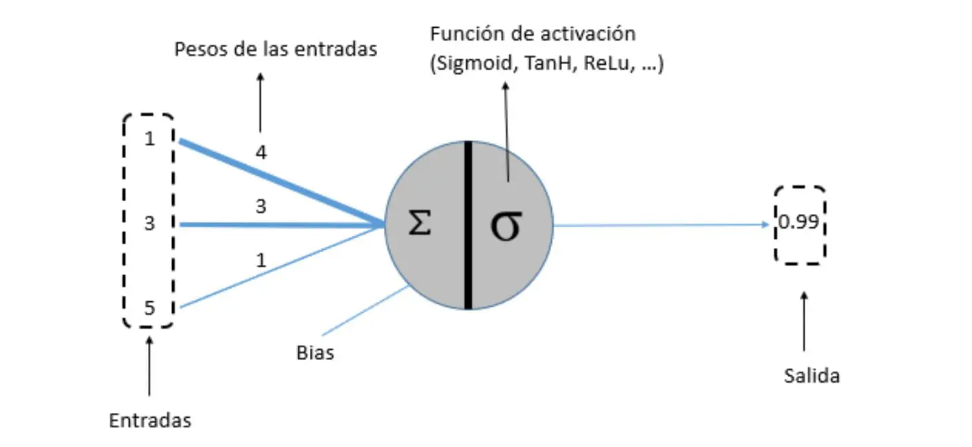
\includegraphics[width=12cm, height=7cm]{nuerona.png}
	\caption{Arquitectura de una neurona.}
\end{figure}

Las neuronas artificiales, reciben una entrada, que pueden ser o bien los datos de entrada para la primera neurona, o la salida de la neurona anterior. Estas entradas tienen unos pesos asociados (que la neuona anterior se ha encargado de proporcionar) y la suma de los valores de entrada multiplicado por sus pesos son los que re procesas en el interior de la célula mediante una función de activación, que nos devuelve el valor de salida de la neurona. A continuación vamos ilustramos las funciones de activación más comunes:

\begin{itemize}
	\item \textbf{Rectified linear unit(Relu)}: La función de activación ReLu aplica una transformación no lineal muy simple, activa la neurona solo si el input está por encima de cero. Mientras el valor de entrada está por debajo de cero, el valor de salida es cero, pero cuando es superior de cero, el valor de salida aumenta de forma lineal con el de entrada.
	
	$$ ReLU(x) = max(x,0) $$
	
	\item \textbf{Softmax}: La función Softmax transforma las salidas a una representación en forma de probabilidades, de tal manera que el sumatorio de todas las probabilidades de las salidas de 1.
	
	$$ \text{Sea } f(x) = ln[1+exp(x)]  \text{ entonces } Softmax(x) = \dfrac{f(x)}{1  f(x)} $$
	
	\item \textbf{sigmoid}: a función sigmoide transforma valores en el rango de (-inf, +inf) a valores en el rango (0, 1).
	
		$$ sigmoid(x) = \dfrac{1}{1+exp(-x)} $$ 
	
	\item \textbf{tanh}: La función de activación Tanh, se comporta de forma similar a la función sigmoide, pero su salida está acotada en el rango (-1, 1).
	
	$$ tanh(x) = \dfrac{1 - exp(-2x)}{1-exp(-2x)} $$
	
	
\end{itemize}

\begin{figure}[h!]
	\centering
	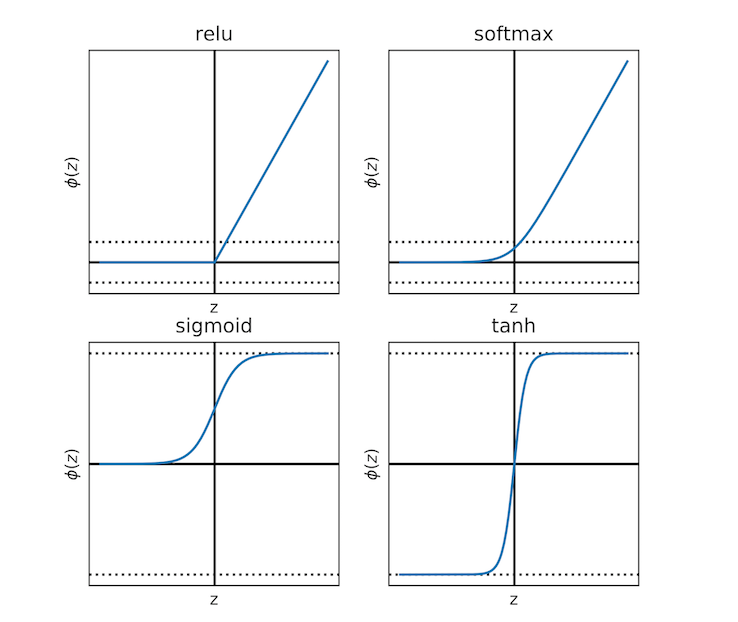
\includegraphics[width=12cm, height=7cm]{funact.png}
	\caption{Arquitectura de una neurona.}
\end{figure}

Para el procesamiento de series temporales, las redes multicapa, son redes neuronales que pueden contar con varias capas, cada una compuesta de una o más neuronas. Las neuronas de una misma capa están desconectadas entre sí, pero están conectadas con las de la capa siguiente y las de la anterior. La primera capa, por la que entran los datos, se denomina \textit{capa de entrada}; a las capas intermedias se les conoce como \textit{capas ocultas} y la última capa es la \textit{capa de salida}. 

Cuando nos enfrentamos al entrenamiento de las redes neuronales también es importante la elección del optimizador que vamos a utilizar. El objetivo del entrenamiendo de las redes es minimizar el coste encontrando los pesos óptimos para las entradas de la red. Para ello utilizamos un algoritmo conocido como backpropagation. Presentamos a continuación un resumen de este algotirmo:

\begin{figure}[h!]
	\centering
	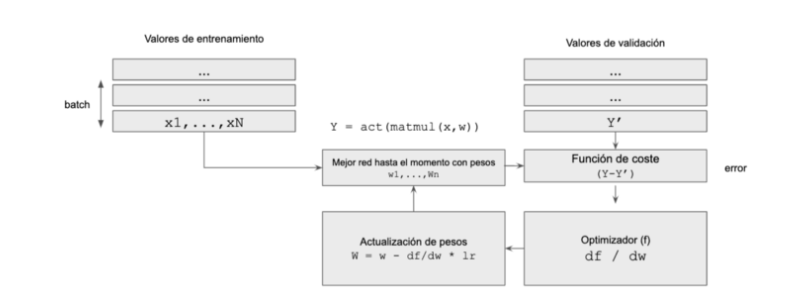
\includegraphics[width=12cm, height=7cm]{backpropagation.png}
	\caption{Algoritmo de backpropagation para el entrenamiento de las redes neuronales.}
\end{figure}


La función de coste o optimizador escogido es el encargado de, minimizar el error obtenido por la red. A continuación, vamos a presentar los principales optimizadores:

\begin{itemize}
	\item \textbf{Stochastic Gradient Descent (SGD)}: 
	
	Como el cálculo de la derivada parcial para cada peso tiene un gran coste, este método estocástico(aleatorio) simplifica el cálculo considerando solo una muestra escogida de forma aleatoria cada vez que realiza el cálculo del gradiente, es decir, pasamos una única muestra, calculamos la función de error asociada y, a partir de esta, el gradiente y los incrementos a aplicar.
	
	El costo de usar SGD es que no necesariamente se obtienen los valores óptimos, pero dado que es menos exigente computacionalmente, se pueden obtener valores lo suficientemente cercanos para lograr un rendimiento adecuado del modelo.
	
	\item \textbf{Adaptative Gradient Estimation (AdaGrad)}: 
	
	Es una extensión del algoritmo SGD. En el algoritmo AdaGrad, no se considera un valor uniforme para todos los pesos, en su lugar mantenemos un factor de entrenamiento específico para cada uno de ellos. Para ello, partimos del factor de entrenamiento inicial, el algoritmo lo escala y adapta para cada dimensión con respecto al gradiente acumulado en cada iteración. Un problema que se presenta es que puede ocurrir que se acumulen valores altos del gradiente al comienzo del entrenamiento, lo que haga que una variable decrezca demasiado rápidamente.
	
	
	\item \textbf{Adaptative Moment Estimation (Adam)}: 
	
	Adam es uno de los algoritmos de optimización más eficientes en el entrenamiento de redes neuronales. En lugar de adaptar la tasa de aprendizaje de los parámetros en función de la media del primer momento, como hemos visto anteriormente, Adam utiliza también la media de los segundos momentos de los gradientes. Este algoritmo calcula la media movil exponencial del gradiente y el gradiente cuadrático. El algoritmo Adam se es una combinación de algoritmos anteriores, por lo que podremos esperar que su rendimiento sea superior.
	

	
	
	
\end{itemize}















\subsubsection{Redes LSTM}

Las redes LSTM o "Long Short-Term Momory" pertenecen al grupo de redes neuronales recurrentes. Esta clase de redes neuronales son las mejores para analizar datos de series temporales ya que tiene conexiones que van retroalimentando las capas, consiguiendo así que no haya pérdida de informacion importante entre la primera neurona y la última.

Podemos considerar que este tipo de red tiene memoria, es decir, tiene una "celda" bloqueada, donde bloqueada significa que puede decidir si eliminar o agregar información al pasar a la siguiente neurona, esto lo hace en función de la importancia que asigna a la información(pesos), que se van aprendiendo conforme avanza el algoritmo.


Como podemos ver en la figura, una unidad LSTM se compone de una entrada y una salida de los datos y una entrada y una salida adicionales. Esta está compuesta por una celda llamada celda de estado (cell state) que se puede definir como una "celda transportadora" a la que podemos añadir o eliminar datos, hace la función de memoria.

Para añadir o quitar datos de esta memoria disponemos de tres compuertas:
la primera, Forget Gate, es la que nos permite eliminar elementos; la segunda, Input Gate, que permite añadir nuevos elementos a la memoria; y por ultimo la Output Gate, o puerta de salida, que nos permite crear el estado oculto actualizado ($c_t$). Estas compuertas son redes neuronales que funcionan como válvulas, utilizan la función sigmoidal para determinar el paso de esta informacion, es decir, si estan completamente abiertas ($\sigma = 1$) permiten el paso de toda la informacion, al contrario cuando estan completamente cerradas ($\sigma = 0$), bloquean el paso de la misma.


\begin{figure}[h!]
	\centering
	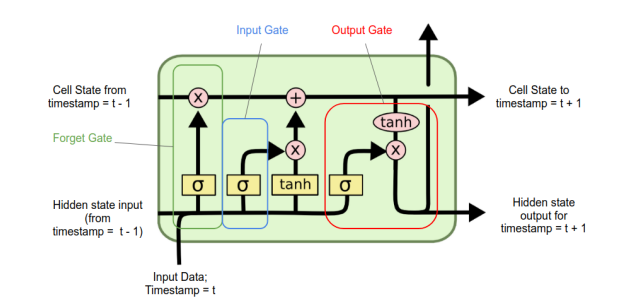
\includegraphics[width=12cm, height=7cm]{imlstm.png}
	\caption{Arquitectura de una celda LSTM.}
\end{figure}


\subsubsection{Redes MLP}

Falta por escribir.



\subsubsection{Redes Neuronales Convolucionales}

Las redes neuronales convolucionales son muy similares a las redes convencionales que se han explicado anteriormente. Lo que las diferencia es que las salidas de estas son imágenes. El objetivo de estas redes es el reconocimiento de objetos en una imagen y para ello se basan en la detección de patrones para su posterior clasificación. Para reconocer estos patrones se realizan en las capas ocultas de la red filtros de convolución, como ahora veremos.

Para realizar el estudio de las imágenes, las capas de una $RNC$ organizan las neuronas en tres dimensiones: anchura, altura y profundidad. Además en estas redes no se impone la condición de que cada una de las neuronas de cada capa tenga que estar conectada con todas las neuronas de la siguiente capa, consiguiendo de esta manera una disminución considerable del número de datos a tratar.

Como sabemos, toda red neuronal se compone de una secuencia de capas y cada capa transforma las neuronas, variando sus pesos, en otras que se ajusten más al modelo. A continuación, vamos a describir las capas más importantes que forman una $RNC$:

\begin{enumerate}
	\item \textbf{INPUT}: esta capa se conforma por la imagen de entrada y se compone de 3 dimensiones: ancho, alto y profundo (la profundidad de entrada es 3, correspondiente a los canales de color RGB).
	\item \textbf{CONV}: es la capa convolucional. En esta capa se consigue llevar a cabo el proceso de detección de patrones en las imágenes. Esta capa realiza la transformación en la dimensión de la profundidad: como hemos visto anteriormente, de entrada una imagen tiene profundidad 3, si aplicamos por ejemplo 12 filtros, tras realizar una convolución, se reduce el tamaño a una única dimensión del canal RGB y posteriormente se transformará en 12 activaciones correspondiéndose cada una a los 12 filtros aplicados. 
	\item \textbf{POOLING}: esta capa tiene la función de realizar un cambio en las dimensiones alto y ancho. Por ejemplo, si el dato que nos llega tiene dimensiones $[32 \times 32 \times 12]$, la salida será $[16 \times 16 \times 12]$.
	\item \textbf{FC}: esta capa es la encargada de computar las probabilidades de cada
	clase, es la última capa de la red y la única que si que está conectada a todas las neuronas de	la capa anterior. El output de esta capa consiste en un vector con tantas componentes como clases hayamos determinado y dicho vector contiene los valores de probabilidad de que la imagen input que hayamos seleccionado pertenezca a una clase u otra.
\end{enumerate}

Es fundamental destacar la distribución de los tipos de filtros a lo largo de la red. Estos
filtros se distribuyen de forma que al principio de la red se sitúan aquellos encargados de la detección de las características más generales y de bajo nivel de la imagen. Al final de la red, se sitúan los filtros encargados de detectar las características de más alto nivel (los detalles mas pequeños y que describen, normalmente, los detalles más característicos de la imagen).



\subsection{Experimentacion}

\subsubsection{Red neuronal utilizando capas Dense}

Las capas \textit{Dense} son las capas que conectan cada una de las neuronas de una capa con todas las salidas de la capa anterior.

\begin{figure}[h!]
	\centering
	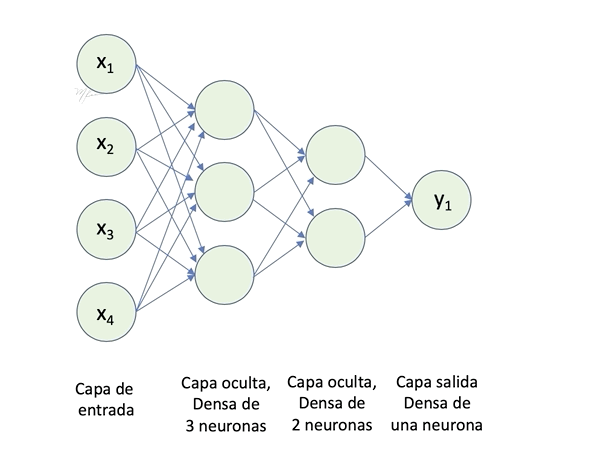
\includegraphics[width=12cm, height=7cm]{imdense1.png}
	\caption{Arquitectura de una celda LSTM.}
\end{figure}

Para comparar los resultados, vamos a modificar el numero de capas, el número de neuronas que tenga cada capa, la función de activación utilizada en cada caso.

Antes de pasar al proceso de entrenamiento de la red, es necesario definir lor parámetros de entrenamiento mediante el método compile que tienen los siguientes parámetros:
\begin{itemize}
	\item Optimizer: metodo de optimización, vamos a probar con el método AdaGrad y el método adam. El método del gradiente estocástico no dió buenos resultados por lo que se ha excluido de las pruebas.
	\item Loss: funcion objetivo a optimizar. Médida disimilaridad entre el valor deseado y el valor predicho por la red. Para nuestras pruebas estimamos el error utilizando el Error Absoluto Medio (mae).
\end{itemize}

Parámetros de la capa Dense:
\begin{itemize}
	\item Units: numero de neuronas, es la dimensión de la salida, y por tanto, la dimensión de entrada de la siguiente neurona.
	\item Activation: Funcion de activación. En nuestro caso vamos a probar con la funcion Rectified Linear Unit (relu).
\end{itemize}


Para evaluar los resultados hemos construido dos modelos diferentes, en uno se ha utilizado la funcion de activación \textit{RELU} con la función de optimización \textit{ADAM}. En la segunda, hemos cambiado el optimizador para utilizar el algoritmo \textit{AdaGrad} y comparar ambos resultados.

Además, se han realizado tres experimentos diferentes, en el que se han modificado el número de capas de la red y el número de neuronas en cada capa. Además, para cada uno de los experimentos vamos a probar con un número diferente de neuronas: 100 neuronas, 64 neuronas y 32 neuronas. Veamos de forma esquemática la estructura de cada una de las redes construidas:

\vspace{2ex}

\begin{tabular}{| c | c | c | c | }
	\hline
	\textbf{CAPA} & \textbf{EXPERIMENTO 1} & \textbf{EXPERIMENTO 2} \\ \hline 
	Capa 1 & Capa Dense/numero de neuronas \textit{n}  & Capa Dense/numero de neuronas \textit{n}   \\ \hline 
	Capa 2 & Capa Dense/numero de neuronas \textit{n/2}  &  Capa Dense/numero de neuronas \textit{n}  \\ \hline 
	Capa 3 & Capa Dense/numero de neuronas \textit{n/3}  & Capa Dense/numero de neuronas \textit{n/2}   \\ \hline 
	Capa 4 & Capa Dense/numero de neuronas \textit{n/4}  &  Capa Dense/numero de neuronas \textit{n/2}  \\ \hline 	
	Capa 5 & Capa Dense/numero de neuronas \textit{1} &  Capa Dense/numero de neuronas \textit{1}  \\ \hline 
\end{tabular}

\vspace{2ex}

\begin{tabular}{| c | c | c | c | }
	\hline
	\centering
	\textbf{CAPA} & \textbf{EXPERIMENTO 3}  \\ \hline 
	Capa 1 & Capa Dense/numero de neuronas \textit{n}    \\ \hline 
	Capa 2 & Capa Dense/numero de neuronas \textit{n/2}    \\ \hline 
	Capa 3 & Capa Dense/numero de neuronas \textit{n/3}   \\ \hline 
	Capa 4 & Capa Dense/numero de neuronas \textit{n/4}   \\ \hline 	
	Capa 5 & Capa Dense/numero de neuronas \textit{n/5}   \\ \hline 
	Capa 6 & Capa Dense/numero de neuronas \textit{n/6}  \\ \hline 
	Capa 7 & Capa Dense/numero de neuronas \textit{n/7}   \\ \hline 
	Capa 8 & Capa Dense/numero de neuronas \textit{n/8}   \\ \hline 	
	Capa 9 &  Capa Dense/numero de neuronas \textit{n/9}  \\ \hline 
	Capa 10 &  Capa Dense/numero de neuronas \textit{1}  \\ \hline 
\end{tabular}

\vspace{2ex}

Por último, como hemos visto anteriormente (adjuntar enlace al apartado de procesamiento de los datos donde explique que hay 3 conjuntos de datos: el simple, añadiendo variables y el último añadiendo algunas variables mas) tenemos tres diferentes conjuntos de datos, en los que hemos ido añadiendo indicadores para comprobar si esto mejora el rendimiento de la red. Añadimos a continuación las tablas donde se indica el error MAE obtenido para cada uno de los modelos citados anteriormente:


\vspace{5ex} 

\begin{tabular}{| c | c | c | }
	\hline
	CONJUNTO DE DATOS 1 & RELU-ADAM & RELU-ADAGRAD \\ \hline 
	Experimento 1 - 100 neuronas & 1421.05 & 1142.68 \\ \hline 
	Experimento 1 - 64 neuronas & 39984.51 & 39984.51 \\ \hline 
	Experimento 1 - 32 neuronas & 39984.51 & 39984.51 \\ \hline
	Experimento 2 - 100 neuronas & 1228.15 & 1358.40 \\ \hline 	
	Experimento 2 - 64 neuronas & 1437.04 & 39984.51 \\ \hline 
	Experimento 2 - 32 neuronas & 39984.51 & 39984.51 \\ \hline 
	Experimento 3 - 100 neuronas & 1719.09 & 1136.02 \\ \hline
	Experimento 3 - 64 neuronas & \textbf{1122.52} & 39984.51 \\ \hline 	
	Experimento 3 - 32 neuronas & 39984.51 & \textbf{1289.93} \\ \hline 
\end{tabular}

\vspace{5ex}

\begin{tabular}{| c | c | c | }
	\hline
	CONJUNTO DE DATOS 2 & RELU-ADAM & RELU-ADAGRAD \\ \hline 
	Experimento 1 - 100 neuronas & 38103.67 & \textbf{996.31} \\ \hline 
	Experimento 1 - 64 neuronas & 985.62 & 1002.96 \\ \hline 
	Experimento 1 - 32 neuronas & \textbf{970.35} & 38103.67 \\ \hline
	Experimento 2 - 100 neuronas & 1045.44 & 1060.34 \\ \hline 	
	Experimento 2 - 64 neuronas & 38103.67 & 1019.05 \\ \hline 
	Experimento 2 - 32 neuronas & 1241.62 & 1049.25 \\ \hline 
	Experimento 3 - 100 neuronas & 38103.67 & 1040.14 \\ \hline
	Experimento 3 - 64 neuronas & 990.04 & 1021.32 \\ \hline 	
	Experimento 3 - 32 neuronas & 979.49 & 1005.72 \\ \hline 
\end{tabular}

\vspace{5ex}

\begin{tabular}{| c | c | c | }
	\hline
	CONJUNTO DE DATOS 3 & RELU-ADAM & RELU-ADAGRAD \\ \hline 
	Experimento 1 - 100 neuronas & 1400.32 & 973.77 \\ \hline 
	Experimento 1 - 64 neuronas & \textbf{1013.68} & \textbf{951.46} \\ \hline 
	Experimento 1 - 32 neuronas & 1060.48 & 1022.98 \\ \hline
	Experimento 2 - 100 neuronas & 2133.38 & 1047.38 \\ \hline 	
	Experimento 2 - 64 neuronas & 37940.60 & 37940.60 \\ \hline 
	Experimento 2 - 32 neuronas & 1239.76 & 1025.83 \\ \hline 
	Experimento 3 - 100 neuronas & 1561.03 & 996.65 \\ \hline
	Experimento 3 - 64 neuronas & 1098.52 & 977.56 \\ \hline 	
	Experimento 3 - 32 neuronas & 37940.60 & 37940.60 \\ \hline 
\end{tabular}



\subsubsection{Red neuronal utilizando capas LSTM}
\subsubsection{Red neuronal utilizando capas MLP}
\subsubsection{Red neuronal utilizando capas Dense-LSTM}
\subsubsection{Red neuronal utilizando capas Dense-MLP}
\subsubsection{Red neuronal utilizando capas LSTM-MLP}

\begin{thebibliography}{999999}
	
Añadir referencias de la parte ya escrita
		
\end{thebibliography}


\end{document}
